% Figure 3: Commutative diagrams for the global and fiberwise scattering
% operators, with the stationary Jost realization and the proof-status legend.
% Authors: Dr. Davide Batic and Dr. Denys Dutykh
%          (Mathematics Department, Khalifa University of Science and
%           Technology, Abu Dhabi, UAE)
\documentclass[tikz,border=6pt]{standalone}
% ============================================================================
% Shared TikZ style for the figures of the Kerr–Dirac two-channel scattering
% manuscript (compiled standalone into ../latex/figures/).
% Authors: Dr. Davide Batic and Dr. Denys Dutykh
%          (Mathematics Department, Khalifa University of Science and
%           Technology, Abu Dhabi, UAE)
%
% Visual language (used consistently across all figures):
%   * horizon channel      : navy  (chH)
%   * spatial-infinity     : teal  (chI)
%   * accents / emphasis   : gold  (acc)
%   * future/out data      : solid arrows
%   * past/in data         : dashed arrows
%   * proved here          : solid box border
%   * imported input       : light-gray filled box
%   * conditional          : dashed box border
% ============================================================================
\usepackage{amsmath,amssymb}
\usetikzlibrary{arrows.meta,positioning,decorations.pathmorphing,calc,matrix}

\definecolor{chH}{HTML}{142D6E}   % horizon channel (navy)
\definecolor{chI}{HTML}{0E6E6E}   % spatial-infinity channel (teal)
\definecolor{acc}{HTML}{9A7A2E}   % gold accent
\definecolor{warm}{HTML}{9C5310}  % sienna (warnings/exclusions)
\definecolor{ltg}{HTML}{F2F2F2}   % light gray fill (imported)

\tikzset{
  outarr/.style={-{Stealth[length=2.6mm]}, line width=0.9pt},
  inarr/.style={-{Stealth[length=2.6mm]}, line width=0.9pt, dashed},
  axis/.style={-{Stealth[length=2.2mm]}, line width=0.6pt, gray!70!black},
  wavyH/.style={chH, decorate, decoration={snake, amplitude=0.45mm, segment length=2.6mm}},
  wavyI/.style={chI, decorate, decoration={snake, amplitude=0.45mm, segment length=2.6mm}},
  proved/.style={draw, line width=0.7pt, rounded corners=2pt, inner sep=4pt},
  imported/.style={draw=gray!60, fill=ltg, line width=0.5pt, rounded corners=2pt, inner sep=4pt},
  conditional/.style={draw, dashed, line width=0.7pt, rounded corners=2pt, inner sep=4pt},
  lab/.style={font=\small},
  slab/.style={font=\footnotesize},
  tlab/.style={font=\scriptsize},
}

\begin{document}
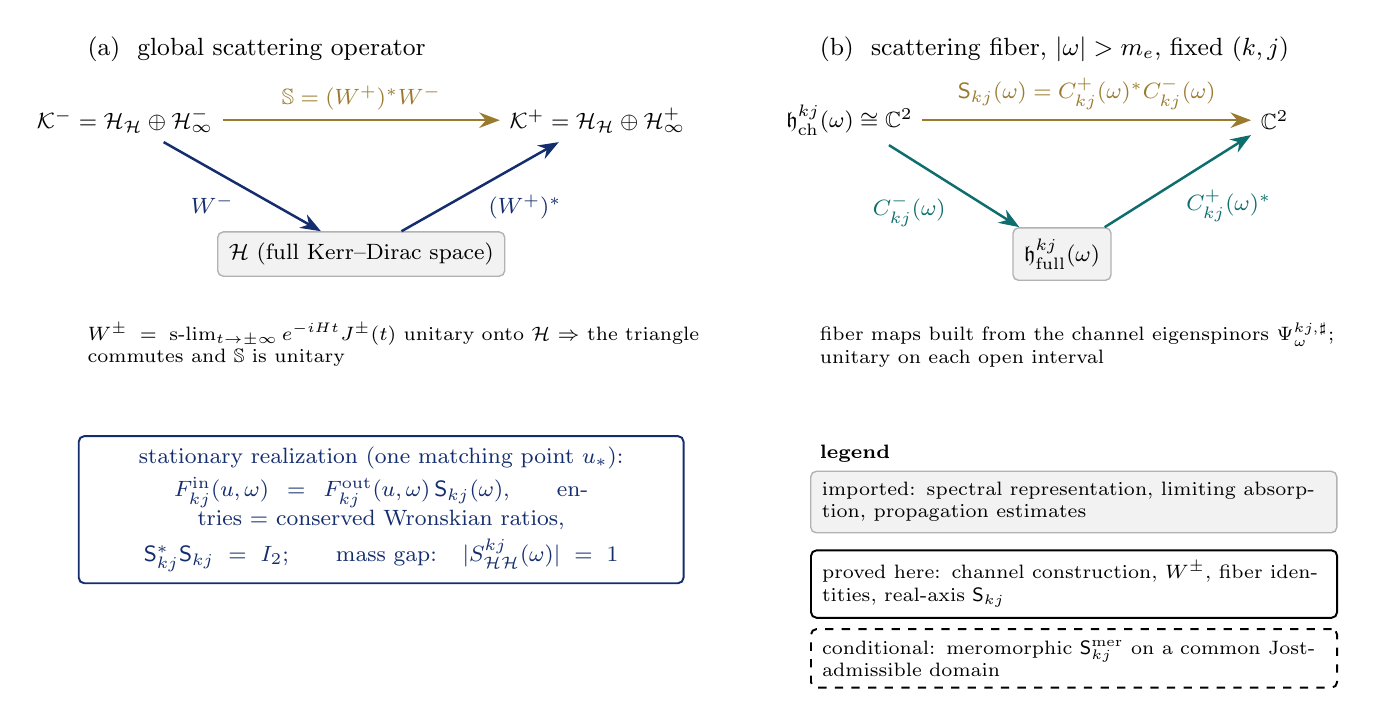
\begin{tikzpicture}[x=1cm,y=1cm]

% ===================== panel (a): global triangle ===========================
\begin{scope}[shift={(0,0)}]
  \node[lab, anchor=west] at (-0.3,2.6) {(a)\ \ global scattering operator};
  \node[slab] (Km) at (0.3,1.7)  {$\mathcal K^-=\mathcal H_{\mathcal H}\oplus\mathcal H_\infty^-$};
  \node[slab] (Kp) at (6.3,1.7)  {$\mathcal K^+=\mathcal H_{\mathcal H}\oplus\mathcal H_\infty^+$};
  \node[imported, slab] (Hf) at (3.3,0.0) {$\mathcal H\ \hbox{(full Kerr--Dirac space)}$};
  \draw[outarr, acc] (Km) -- (Kp) node[midway, above, slab, acc]
    {$\mathbb S=(W^+)^*W^-$};
  \draw[outarr, chH] (Km) -- (Hf) node[midway, below left=-1pt, slab, chH] {$W^-$};
  \draw[outarr, chH] (Hf) -- (Kp) node[midway, below right=-1pt, slab, chH] {$(W^+)^*$};
  \node[tlab, anchor=north west, text width=8.3cm] at (-0.3,-0.75)
    {$W^\pm=\operatorname*{s-lim}_{t\to\pm\infty}e^{-iHt}J^\pm(t)$
     unitary onto $\mathcal H$\ $\Rightarrow$\ the triangle commutes and
     $\mathbb S$ is unitary};
\end{scope}

% ===================== panel (b): fiber triangle ============================
\begin{scope}[shift={(9.3,0)}]
  \node[lab, anchor=west] at (-0.3,2.6) {(b)\ \ scattering fiber, $|\omega|>m_e$, fixed $(k,j)$};
  \node[slab] (fm) at (0.2,1.7)  {$\mathfrak h^{kj}_{\rm ch}(\omega)\cong\mathbb C^2$};
  \node[slab] (fp) at (5.6,1.7)  {$\mathbb C^2$};
  \node[imported, slab] (ff) at (2.9,0.0) {$\mathfrak h^{kj}_{\rm full}(\omega)$};
  \draw[outarr, acc] (fm) -- (fp) node[midway, above, slab, acc]
    {$\mathsf S_{kj}(\omega)=C^+_{kj}(\omega)^*C^-_{kj}(\omega)$};
  \draw[outarr, chI] (fm) -- (ff) node[midway, below left=-1pt, slab, chI] {$C^-_{kj}(\omega)$};
  \draw[outarr, chI] (ff) -- (fp) node[midway, below right=-1pt, slab, chI] {$C^+_{kj}(\omega)^*$};
  \node[tlab, anchor=north west, text width=6.6cm] at (-0.3,-0.75)
    {fiber maps built from the channel eigenspinors
     $\Psi^{kj,\sharp}_\omega$; unitary on each open interval};
\end{scope}

% ===================== bottom row: Jost realization + legend ================
\begin{scope}[shift={(0,-2.6)}]
  \node[proved, chH, slab, align=center, anchor=north west, text width=7.4cm] at (-0.3,0.3)
    {stationary realization (one matching point $u_*$):\\[0.8mm]
     $F^{\rm in}_{kj}(u,\omega)=F^{\rm out}_{kj}(u,\omega)\,\mathsf S_{kj}(\omega)$,\qquad
     entries $=$ conserved Wronskian ratios,\\[0.8mm]
     $\mathsf S_{kj}^*\mathsf S_{kj}=I_2$;\qquad mass gap:
     $\;|S^{kj}_{\mathcal H\mathcal H}(\omega)|=1$};
  \node[tlab, anchor=north west] at (9.0,0.30) {\textbf{legend}};
  \node[imported, tlab, anchor=north west, text width=6.4cm] at (9.0,-0.15)
    {imported: spectral representation, limiting absorption, propagation estimates};
  \node[proved, tlab, anchor=north west, text width=6.4cm] at (9.0,-1.15)
    {proved here: channel construction, $W^\pm$, fiber identities, real-axis $\mathsf S_{kj}$};
  \node[conditional, tlab, anchor=north west, text width=6.4cm] at (9.0,-2.15)
    {conditional: meromorphic $\mathsf S^{\rm mer}_{kj}$ on a common Jost-admissible domain};
\end{scope}

\end{tikzpicture}
\end{document}
